\section{Results}
\label{sec:experiments}

\begin{table}[tb]
  \begin{footnotesize}
    \begin{center}
%        \scalebox{0.96}{
          % \begin{tabular}{l | p{2cm} | p{2cm} | p{2cm}}
          \begin{tabular}{l | r | r | r}
             & \textbf{random} & \textbf{jump} & \textbf{around-right} \\ \hline
             LSTM & 99.8 & 1.2 & 2.5$\pm$2.7 \\
             GRU & \textbf{100.0}$\pm$0.0 & 12.5$\pm$6.6 & --  \\
             \hline
              CNN & \textbf{100.0}$\pm$0.0 & \textbf{69.2}$\pm$8.2 & \textbf{56.7}$\pm$10.2 \\
          \end{tabular} 
%    }
    \end{center}
  \end{footnotesize}
  \caption{Test accuracy (\%) on SCAN splits (means across 5 seeds,
    with standard deviation if available). Top LSTM results from
    \newcite{Lake:Baroni:2017}/\newcite{Loula:etal:2018}, GRU from
      \newcite{Bastings:etal:2018}.}
\label{table:main_results} 
\end{table}

Our main results are in Table \ref{table:main_results}. CNNs, like
RNNs, succeed in the \emph{random} split, and achieve much higher accuracy (albeit still far from being perfect)  in the challenging \emph{jump} and \emph{around-right}
splits.

The SCAN tasks should be easy for a system that learned the right
composition rules. Perhaps, CNNs do not achieve 100\% accuracy because
they only learned a subset of the necessary rules. For example, they
might correctly interpret the new expression \emph{jump twice} because
they induced a \emph{X twice} rule at training time, but fail
\emph{jump thrice} because they missed the corresponding \emph{X
  thrice} rule. Since SCAN semantic composition rules are associated
with single words in input commands, we can check this hypothesis by
looking at error distribution across input words. It turns
out (Fig.~\ref{fig:error_distributions}) that errors are not
associated to specific input commands. Error proportion is instead relatively
stable across command words. Direct inspection reveals no traces of
systematicity: errors cut across composition rules. Indeed, we
often find minimal pairs in which changing one action verb with
another (distributionally equivalent in SCAN) turns a correctly
executed command into a failed one. For example, in the \emph{jump}
split, the CNN correctly executes \emph{jump left after walk}, but
fails \emph{jump left after run} (jumping is
forgotten). Analogously, in the \emph{around-right} split, \emph{run
  around right} is correctly executed, but ``\emph{walk around
  right}'' is not (the network stops too early).
\begin{figure}[tb]
    \centering
    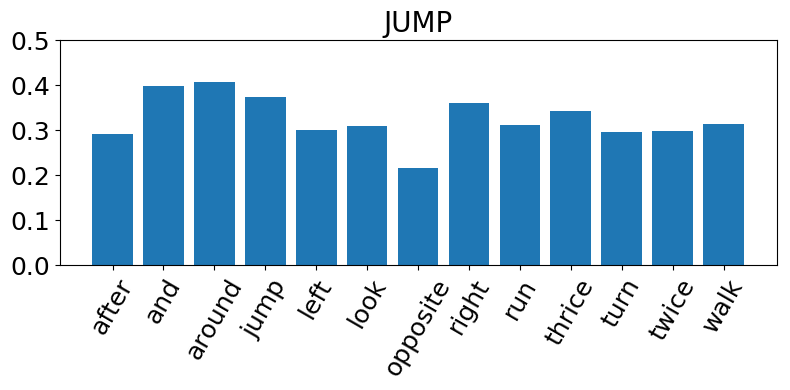
\includegraphics[width=.45\textwidth,keepaspectratio]{figures/jump_error_dist.png}
    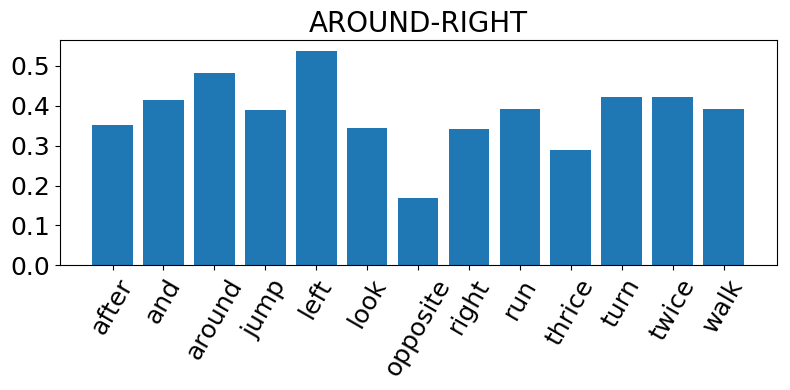
\includegraphics[width=.45\textwidth,keepaspectratio]{figures/template_error_dist.png}
    \caption{Proportion of commands with a certain command word (over total commands with that word) wrongly executed by best CNNs.}
    \label{fig:error_distributions}
\end{figure}
\paragraph{Robustness} Fig.~\ref{fig:exp1} shows a big difference in
stability between \emph{random} and the other splits across top
hyperparameter configurations. The \emph{random} results are very
stable. \emph{Jump} accuracy is relatively stable across
hyperparameters, but has large variance across initialization
seeds. For the most challenging \emph{around-right} split, we observe
instability both across seeds and hyperparameters (although even the
lowest end of the reported accuracies is well above best RNN
performance in the corresponding experiments). Another question is
whether the best configurations are shared, or each split requires an
\emph{ad-hoc} hyperparameter choice. We find that there are configurations
that achieve good performance across the splits. In particular, the
\emph{best overall configuration}, found by minimizing ranks across
splits, has 0.01 learning rate, 25-tokens batch size, 0.25
dropout, 6 layers, 512 layer dimensionality, and kernels of width
5. Such model was 13th best (of about 2.5K explored) on the
\emph{random} split (with mean cross-seed accuracy of 99.92\%, off
by 0.05\% from top configuration), 32th on the \emph{jump} split
(60.67\% mean accuracy, off by 8.62\%), and 2nd in the
\emph{around-right} split (mean 53.25\% accuracy, off by 3.45\%).

\begin{figure}[tb]
    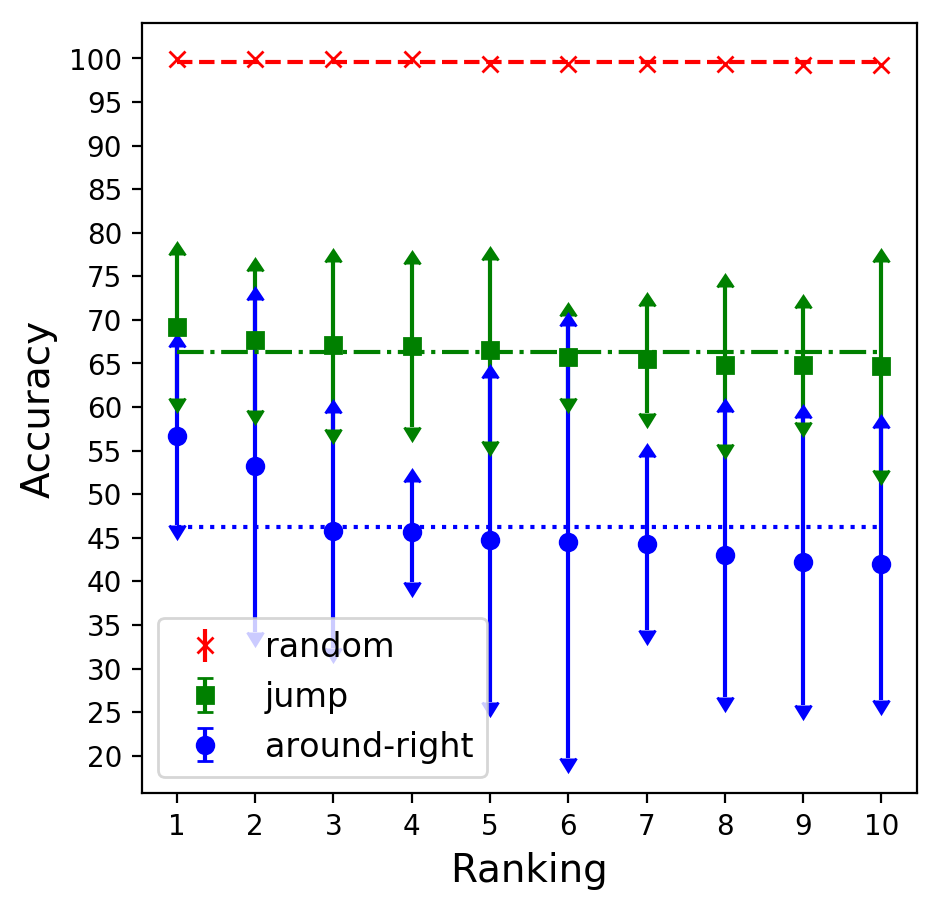
\includegraphics[width=.45\textwidth,keepaspectratio]{figures/accuracies_all_splits.png}
    \centering
    \caption{Accuracies (\%) of top-10 models on \emph{random}, \emph{jump} and \emph{around-right}. Arrows
      denote standard deviations, dashed lines average accuracy across top-10.
      % \mb{means across what? Also, it would be better if
      %legend order was random/jump/around-right}
      }
    \label{fig:exp1}
\end{figure}

\paragraph{Kernel width}
\label{subsec:exp2}

One important difference between recurrent and convolutional
architectures is that CNN kernel
width imposes a strong prior on the window of elements to be
processed together. We conjecture that relatively wide encoder and
decoder widths, by pushing the network to keep wider
contexts into account, might favour the acquisition of template-based
generalizations, and hence better compositionality. To investigate
this, we varied encoder and decoder widths of the best-overall model
between 1 and 5.\footnote{At least on the encoder side, larger widths
  seem excessive, as the longest commands are 9-word-long.}


\begin{figure*}[tb]
    \centering
    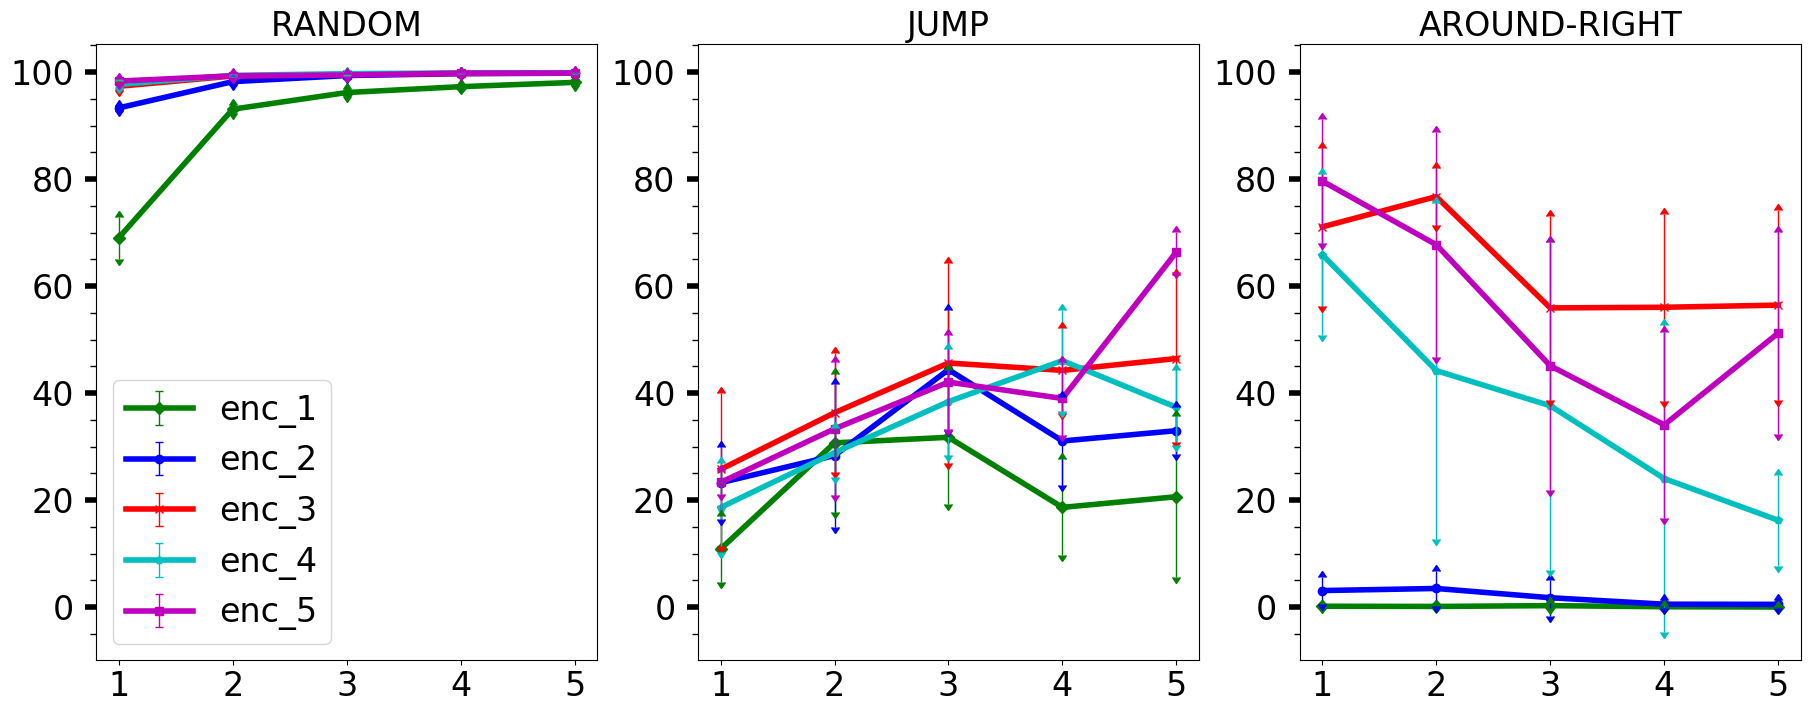
\includegraphics[width=\textwidth,keepaspectratio]{figures/kernel_exp.png}
    \caption{Mean accuracies (\%) across 5 seeds, in function of decoder (x axis) and encoder (colors) kernel widths. Arrows denote standard deviations. Best viewed in color.
    %More natural order would be random/jump/around-right.
%    \mb{Also crop actual file and enlarge figure.}
    }
    \label{fig:kernel_exp}
\end{figure*}

Fig.~\ref{fig:kernel_exp} shows that the \emph{random} split confirms
our expectations, as both wider encoder and decoder windows improve
performance. The \emph{jump} results follow the same trend, although
in a less clear-cut way. Still, the narrowest encoder-decoder
combination has the worst performance, and the widest one the top
one. For the \emph{around-right} split, it is also better to use the
widest encoder, but top performance is achieved with the
\emph{narrowest} decoder (width$=$1). Indeed, with the narrow decoder
we obtain \emph{around-right} accuracies that are even above the
absolute-best \emph{jump}-split performance. Since the novel output
templates in the \emph{around-right} split are by construction long
(they involve executing an \emph{around} command that requires
repeating an action 4 times), we would have rather expected models
keeping track of a larger decoding window to fare better, particularly
in this case. We tried to gain some insight on the attested behaviour
by looking at performance distribution in function of input and output
length, failing to detect different patterns in the wide-decoder
\emph{jump} model vs.~the narrow-decoder \emph{around-right} model
(analysis not reported here for space reasons). Looking qualitatively
at the errors, we note that, for both splits, the narrower decoder
tends to skip trajectory sub-chunks (e.g., executing ``\emph{jump
  around right}'' with 3 instead of 4 right turns followed by jumps),
whereas the wider kernel is more likely to substitute actions (e.g.,
turning left instead of right) than undershooting the length. This
impressionistic observation is supported by the fact that, for both
splits, the narrow-kernel errors have considerably larger variance
than the wide-kernel errors with respect to ground-truth length,
indicating that, with narrow decoder kernel, the model is less stable in terms of output sequence length. This, however, only confirms our
 conjecture that a wider decoder kernel helps length management.
We still have no insight on why the narrower kernel should be better on
the \emph{around-right split}.
\paragraph{Multi-layer attention}
\label{subsec:exp3}

The fairseq CNN has attention from all layers of the
decoder. Is the possibility to focus on different aspects of the input
while decoding from different layers crucial to its better
generalization skills? Fig.~\ref{fig:exp3} reports
accuracies when applying attention from a subset of the 6
layers only. The \emph{random} split differences are minimal,
but ablating attentions greatly affects performance on the
compositional splits (although, in both cases, there is a single ablated
configuration that is as good as the full setup).

\begin{figure}[tb]
    \centering
    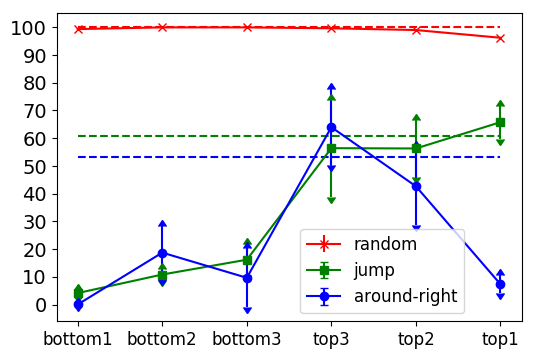
\includegraphics[width=.48\textwidth,keepaspectratio]{figures/attention_exp.png}
    \caption{Accuracy (\%) of overall-best model with attention
      only from first layer (\emph{bottom1}), first two layers
      (\emph{bottom2}), \ldots, last two layers (\emph{top2}), top
      layer only (\emph{top1}). Means and standard deviations across 5
      seeds. Dashed lines show full multi-layer attention results.}
    \label{fig:exp3}
\end{figure}

